\documentclass[10pt,twocolumn,letterpaper]{article}

\usepackage{semml}
\usepackage{times}
\usepackage{epsfig}
\usepackage{graphicx}
\usepackage{amsmath}
\usepackage{amssymb}

% Include other packages here, before hyperref.
\usepackage{amsthm}
\usepackage{listings}
\usepackage{braket}
\usepackage{algpseudocodex}
\usepackage{algorithmicx}

% If you comment hyperref and then uncomment it, you should delete
% egpaper.aux before re-running latex.  (Or just hit 'q' on the first latex
% run, let it finish, and you should be clear).
\usepackage[breaklinks=true,bookmarks=false]{hyperref}
\usepackage{lstmisc}

\semmlfinalcopy % *** Uncomment this line for the final submission

\def\semmlPaperID{****} % *** Enter the SemML Paper ID here
\def\httilde{\mbox{\tt\raisebox{-.5ex}{\symbol{126}}}}

% Pages are numbered in submission mode, and unnumbered in camera-ready
%\ifsemmlfinal\pagestyle{empty}\fi
\setcounter{page}{1}
\begin{document}

%%%%%%%%% TITLE
\title{Unsupervised Learning: Improving the K-Means Algorithm}

\author{Juri Kembügler\\
Friedrich-Alexander-Universität\\
Erlangen, Germany\\
{\tt\small\href{mailto:juri.kembuegler@fau.de}{juri.kembuegler@fau.de}}
% For a paper whose authors are all at the same institution,
% omit the following lines up until the closing ``}''.
% Additional authors and addresses can be added with ``\and'',
% just like the second author.
% To save space, use either the email address or home page, not both
%\and
%Second Author\\
%Institution2\\
%First line of institution2 address\\
%{\tt\small secondauthor@i2.org}
}

\maketitle
%\thispagestyle{empty}

%%%%%%%%% ABSTRACT
\begin{abstract}
    The ABSTRACT is to be in fully-justified italicized text, at the top
    of the left-hand column, below the author and affiliation
    information. Use the word ``Abstract'' as the title, in 12-point
    Times, boldface type, centered relative to the column, initially
    capitalized. The abstract is to be in 10-point, single-spaced type.
    Leave two blank lines after the Abstract, then begin the main text.
    Look at previous SemML abstracts to get a feel for style and length.
\end{abstract}

%%%%%%%%% BODY TEXT

\section{Introduction}\label{sec:introduction}
% TODO: Add sources to the Introduction

Digitalization has permeated various aspects of our daily lives, from sports
and fitness tracking to entertainment platforms such as YouTube and Twitch, as
well as digital newspaper consumption. A key consequence of this transformation
in recent years is the vast amount of data generated by computers, smartphones,
smartwatches and other IoT devices. In 2010, the global data volume was
%TODO: it was projected?
approximately two zettabytes, whereas by 2024, it is projected to reach around
150 zettabytes (1 zettabyte $\approx10^{21}$ bytes). Notably, since the onset
of the global COVID-19 pandemic in 2020, the growth rate of data generation and
consumption has accelerated significantly~\cite{IDC_Statista_2024}. Thus,
extracting meaningful insights from this data requires efficient and robust
algorithms.

To extract meaningful insights from this data, Machine Learning has become an
essential tool. Machine Learning algorithms enable systems to identify patterns
and make decisions based on data. One important branch of Machine Learning is
unsupervised learning, where algorithms uncover hidden structures in data
without predefined labels. A fundamental technique in this domain is
clustering, with K-Means being one of the most widely used methods. However,
the performance of K-Means is highly dependent on the initial choice of
centroids.
% TODO: Source??? And maybe do not mention K-means and unsupervised learning herer?

\subsubsection{Contributions}

In this article, we make the following contributions:
%TODO: should we call this "contributions"?? Maybe

\begin{itemize}
    \item We provide an overview of clustering as an unsupervised Machine Learning
          technique.
    \item We analyze the K-Means algorithm, discussing its methodology and limitations.
    \item We present K-Means++ as a well-known and a statistical relatively new, less
          commonly used approach to improve K-Means.
    \item (Hopefully we also find an improvment for the statistical approach)
    \item We evaluate the performance of these improvements on various datasets.
\end{itemize}

%-------------------------------------------------------------------------

\section{Background and Related Work}\label{sec:background-and-related-work}

%------------------------------------------------------------------------

\subsection{Machine Learning techniques}\label{subsec:machine-learning-techniques}

Machine learning leverages statistical methods, mathematical models, and
numerical techniques to extract meaningful patterns from data, enabling tasks
such as summarization, clustering, visualization, and prediction. The learning
process is generally categorized into two main paradigms: \textit{supervised}
and \textit{unsupervised learning}~\cite{deuschle2019}.

%-------------------------------------------------------------------------
% TODO: Check Plagiat on kushawahAndYadav2016

\subsubsection{Supervised Learning}\label{subsubsec:supervised-learning}

A supervised training technique is the technique where we consider both the
input and the output before using our machine learning model. We then attempt
to use our model to make statements or predictions about new unseen
data~\cite{deuschle2019}. Known techniques are neural networks, several layers
perception and decision trees~\cite{kushawahAndYadav2016}.

%------------------------------------------------------------------------

\subsubsection{Unsupervised Learning}\label{subsubsec:unsupervised-learning}

An unsupervised training technique is the technique where we now only consider
a dataset of only the inputs. We then use our Machine Learining model, to
somewhat describe, summarize or categorize our data~\cite{deuschle2019}. Known
techniques are non-identical types of clustering, amplitude and normalization,
k-means and self-organising maps~\cite{kushawahAndYadav2016}.

%------------------------------------------------------------------------

\subsection{Clustering}\label{subsec:clustering}

The objective of clustering is to group similar objects based on their
characteristics. The concept of '\textit{similarity}' implies the use of a
distance metric to quantify the relationships between data points. One of the
most widely used distance metrics is the L2 norm (Euclidean
distance)~\cite{deuschle2019}. Alternative metrics such as the L1 norm,
Itakura-Saito or Bregman distance can also be employed, depending on the
specific application and data properties~\cite{Jain2010651}.

Clustering is mainly used to get an overview of data, to summarize it and to
simplify human interpretation by categorizing the data and highlighting
characteristics that distinguish the data points. However, it can also be used
as a preprocessing step for other methods (e.g. feature creation for supervised
learning)~\cite{Jain2010651}.

%------------------------------------------------------------------------

\subsubsection{Common clustering algorithms}\label{subsubsec:common-clustering-algorithms}

Overall, clustering algorithms can be classified into two categories:
\textit{hierarchical} and \textit{partitional} algorithms. Hierarchical
algorithms build clusters by recursively merging related data points, whereas
partitional algorithms divide the dataset into distinct clusters
simultaneously~\cite{Ezugwu2022104743,Jain2010651}.

Hierarchical clustering methods include \textit{agglomerative} approaches (such
as single-, complete-, and average-linkage) and \textit{divisive} (e.g.,
monothetic and polythetic) clustering. Partitional techniques, on the other
hand, encompass algorithms such as \textit{K-Means}, \textit{Genetic
    Algorithms}, \textit{Gaussian Mixture Models}, \textit{Fuzzy C-Means}, and
\textit{DBSCAN}~\cite{Ezugwu2022104743}.

%------------------------------------------------------------------------

\subsection{Types of Clusters}\label{subsec:types-of-clusters}

Kapil Joshi \etal~\cite{Joshi2015} divide clusters into four categories. In the
general literature on cluster analysis, it is discussed that the choice of the
appropriate algorithm depends on the underlying cluster
structure~\cite{Ezugwu2022104743}. For example, density-based methods such as
DBSCAN are particularly suitable for non-convex clusters~\cite{Bhargav2016},
while k-Means works particularly well for spherical
clusters~\cite{Jain2010651}.

\theoremstyle{definition}
\newtheorem{definition}{Definition}[subsubsection]

\subsubsection{Definitions of cluster types~\cite{Joshi2015}}

\begin{definition}[Well-separated clusters]
    \label{def:well-separated}
    A point in a cluster is closer or more similar to any point in the same cluster
    as to a point in another cluster.
\end{definition}

\begin{definition}[Centre-based clusters]
    \label{def:centre-based}
    A point in a cluster is closer or more similar to the ‘centre’ of this cluster
    than to the centre of another cluster.
\end{definition}

\begin{definition}[Contiguous clusters]
    \label{def:contiguous}
    A point in a cluster is closer to one or more points in the same cluster as to
    any other point not in the cluster.
\end{definition}

\begin{definition}[Density-based clusters]
    \label{def:density-based}
    A cluster is a dense region of points separated from other high-density
    regions by low-density regions.
\end{definition}

%------------------------------------------------------------------------

\section{K-Means}\label{sec:k-means}

In contrast to other algorithms, K-Means was discovered independently in
various research fields, first by Steinhaus (1956) and Lloyd (proposed 1957;
published 1982) and later by Ball and Hall (1965) and MacQueen
(1967)~\cite{Jain2010651}.

Despite variations in their implementation, all K-Means algorithms follow the
same fundamental procedure for partitioning data into clusters. Given an input
dataset represented as a $n \times d$ matrix — where $n$ is the number of data
points and $d$ the number of features — K-Means requires the number of desired
clusters, a similarity metric and an initialization strategy. The algorithm
proceeds as follows:
\begin{enumerate}
    \item Select the initial $k$ cluster centres (centroids) based on the initialization
          method. This selection of centroids now acts as a starting point for the
          further procedure.
    \item Assign each data point to the nearest cluster based on our similarity metric
          (e.g. Euclidean norm).
    \item Update the centroids based on the assignments from step 2, where we select the
          mean of all points assigned to a cluster as the new centroid of that cluster.
    \item Repeat steps 2 and 3 until the clusters converge. So the data points no longer
          change their assigned clusters within an iteration.
\end{enumerate}
An illustration of this process is provided in Figure
~\ref{fig:kmeans-procedure}. However, they differ subtly in their objectives
and approaches. For example, unlike Lloyd's algorithm, which updates centroids
only after all data points have been reassigned, MacQueen's algorithm performs
incremental updates, adjusting the affected cluster’s centroid immediately when
a data point moves from one cluster to another~\cite{Morissette2013}.

\begin{figure}[t]
    \begin{center}
        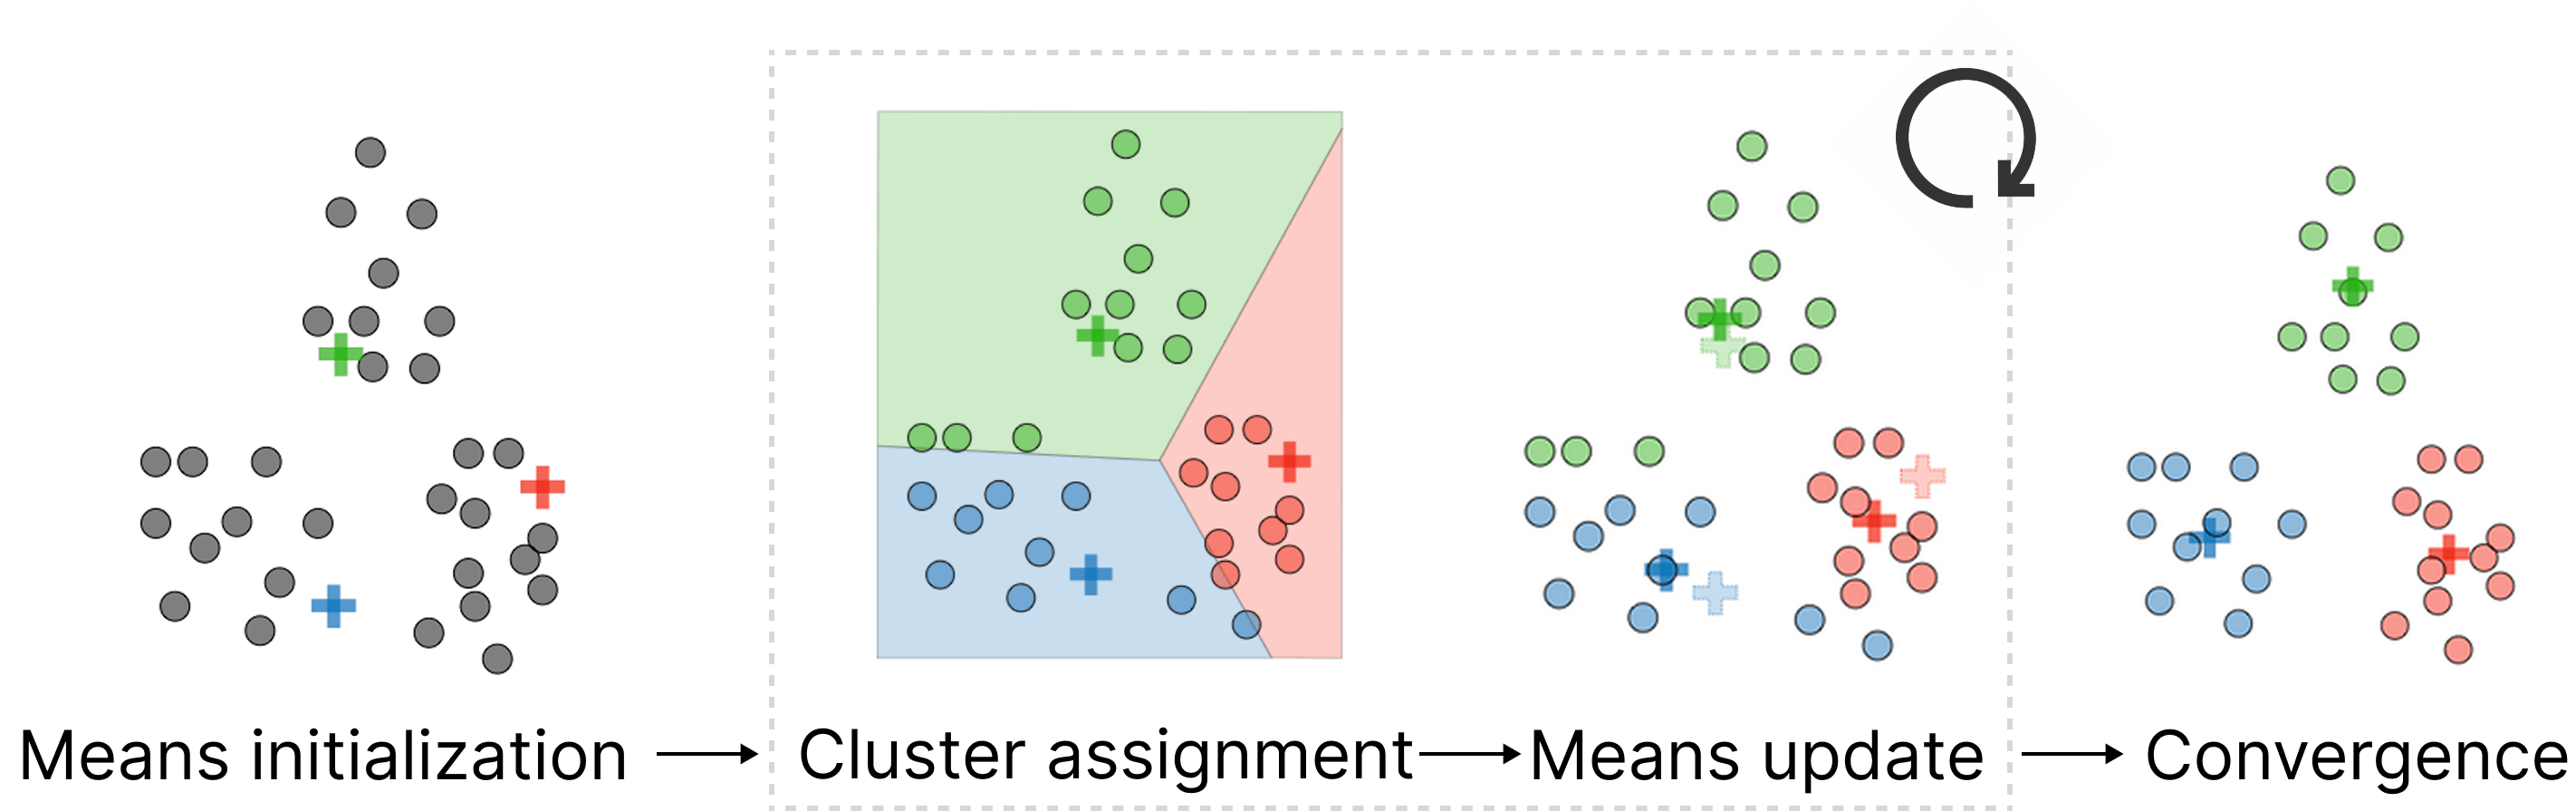
\includegraphics[width=0.9\linewidth]{figures/K-Means procedure}
    \end{center}
    \caption{K-Means procedure visualised \cite{Amidi2018}.}
    \label{fig:kmeans-procedure}
\end{figure}

%------------------------------------------------------------------------

\subsection{Lloyd's algorithm}\label{subsec:procedure-and-lloyd's-algorithm}

One of the most widely used implementations of K-Means is Lloyd’s
algorithm~\cite{deuschle2019}, which iteratively refines cluster assignments
and centroids through a simple yet effective approach. Given a dataset
$X=\set{x_i}_{i=1}^n$ of $d$-dimensional points, the goal is to iteratively
refine the centroids $C=\Set{\mu_i}_{i=1}^k$ to partition the data into $k$
clusters. The assignment of data points to clusters is encoded by a
responsibility vector $R\in\Set{0,1}^{n\times k}$, where $r_{nk}=1$ indicates
that point $x_i$ belongs to cluster $k$, and $0$ otherwise.

To quantify clustering quality, we define the loss function, also known as the
\textit{sum-of-squared errors (SSE)}, as the sum of squared distances between
data points and their assigned centroids:
\begin{equation}
    \label{eq:lloyds-loss}
    \mathcal{L} = \sum_{n=1}^{N} \sum_{c=1}^{k} r_{nc} \|x_n - \mu_c\|^2.
\end{equation}
To minimize $\mathcal{L}$, Lloyd's algorithm iterates between two steps~\cite{deuschle2019, FRANTI201995}:
\begin{enumerate}
    \item \textbf{Assignment Step:} Each data point is assigned to the nearest centroid by updating the responsibility vector:
          \begin{equation}
              \label{eq:lloyds-res-vec}
              r_{nc} =
              \begin{cases}
                  1, & \text{if } c = \underset{c'}{\arg\min} \|x_n - \mu_{c'}\| \\
                  0, & \text{otherwise.}
              \end{cases}
          \end{equation}
    \item \textbf{Update Step:} The cluster centroids are recomputed as the mean of all assigned points:
          \begin{equation}
              \label{eq:min-lloyds-loss}
              \mu_c' = \frac{\sum_{n=1}^{N} r_{nc} x_n}{\sum_{n=1}^{N} r_{nc}}
          \end{equation}
\end{enumerate}
These steps repeat until the assignments $R$ no longer change, indicating
convergence. Since the loss function $\mathcal{L}$ is non-increasing at each
iteration, the algorithm is guaranteed to reach a local minimum, though not
necessarily the global optimum.

%------------------------------------------------------------------------

\subsection{Problems and limitations}\label{subsec:problems-and-limitations}

Despite its simplicity and efficiency, K-Means has several
limitations~\cite{Ezugwu2022104743, FRANTI201995, Jain2010651}. Since it relies
on distance calculations, standardizing data is often necessary to ensure equal
feature contributions~\cite{Morissette2013}. The algorithm’s sensitivity to the
choice of $k$ and centroid initialization can significantly impact performance.
This section explores these challenges and strategies to address them.

%------------------------------------------------------------------------

\subsubsection{Choose $k$}

One of the few adjustable parameters in Lloyd's algorithm, apart from the
initialization method, is the number of clusters $k$. Examining the loss
function in Equation~(\ref{eq:lloyds-loss}), we observe that a smaller number
of clusters generally results in a higher loss, as data points are assigned to
fewer centroids. Conversely, the loss decreases as $k$ increases, reaching its
minimum when each data point forms its own cluster. However, this solution is
not meaningful, as it eliminates the concept of clustering altogether
~\cite{deuschle2019}. Since there is no universally optimal choice for $k$,
Jain~\cite{Jain2010651} suggests running the algorithm with multiple values of
$k$ and selecting the most significant one based on evaluation criteria.

A widely used heuristic for determining $k$ is the \textit{elbow method}. This
approach involves plotting the loss function against $k$ and identifying the
point where the decrease in loss slows significantly — forming an 'elbow' in
the curve (see Figure~\ref{fig:elbow-plot}). The fundamental concept behind
this method is that above a certain $k$, additional clusters result in
diminishing returns in loss reduction~\cite{deuschle2019}.

\begin{figure}[t]
    \begin{center}
        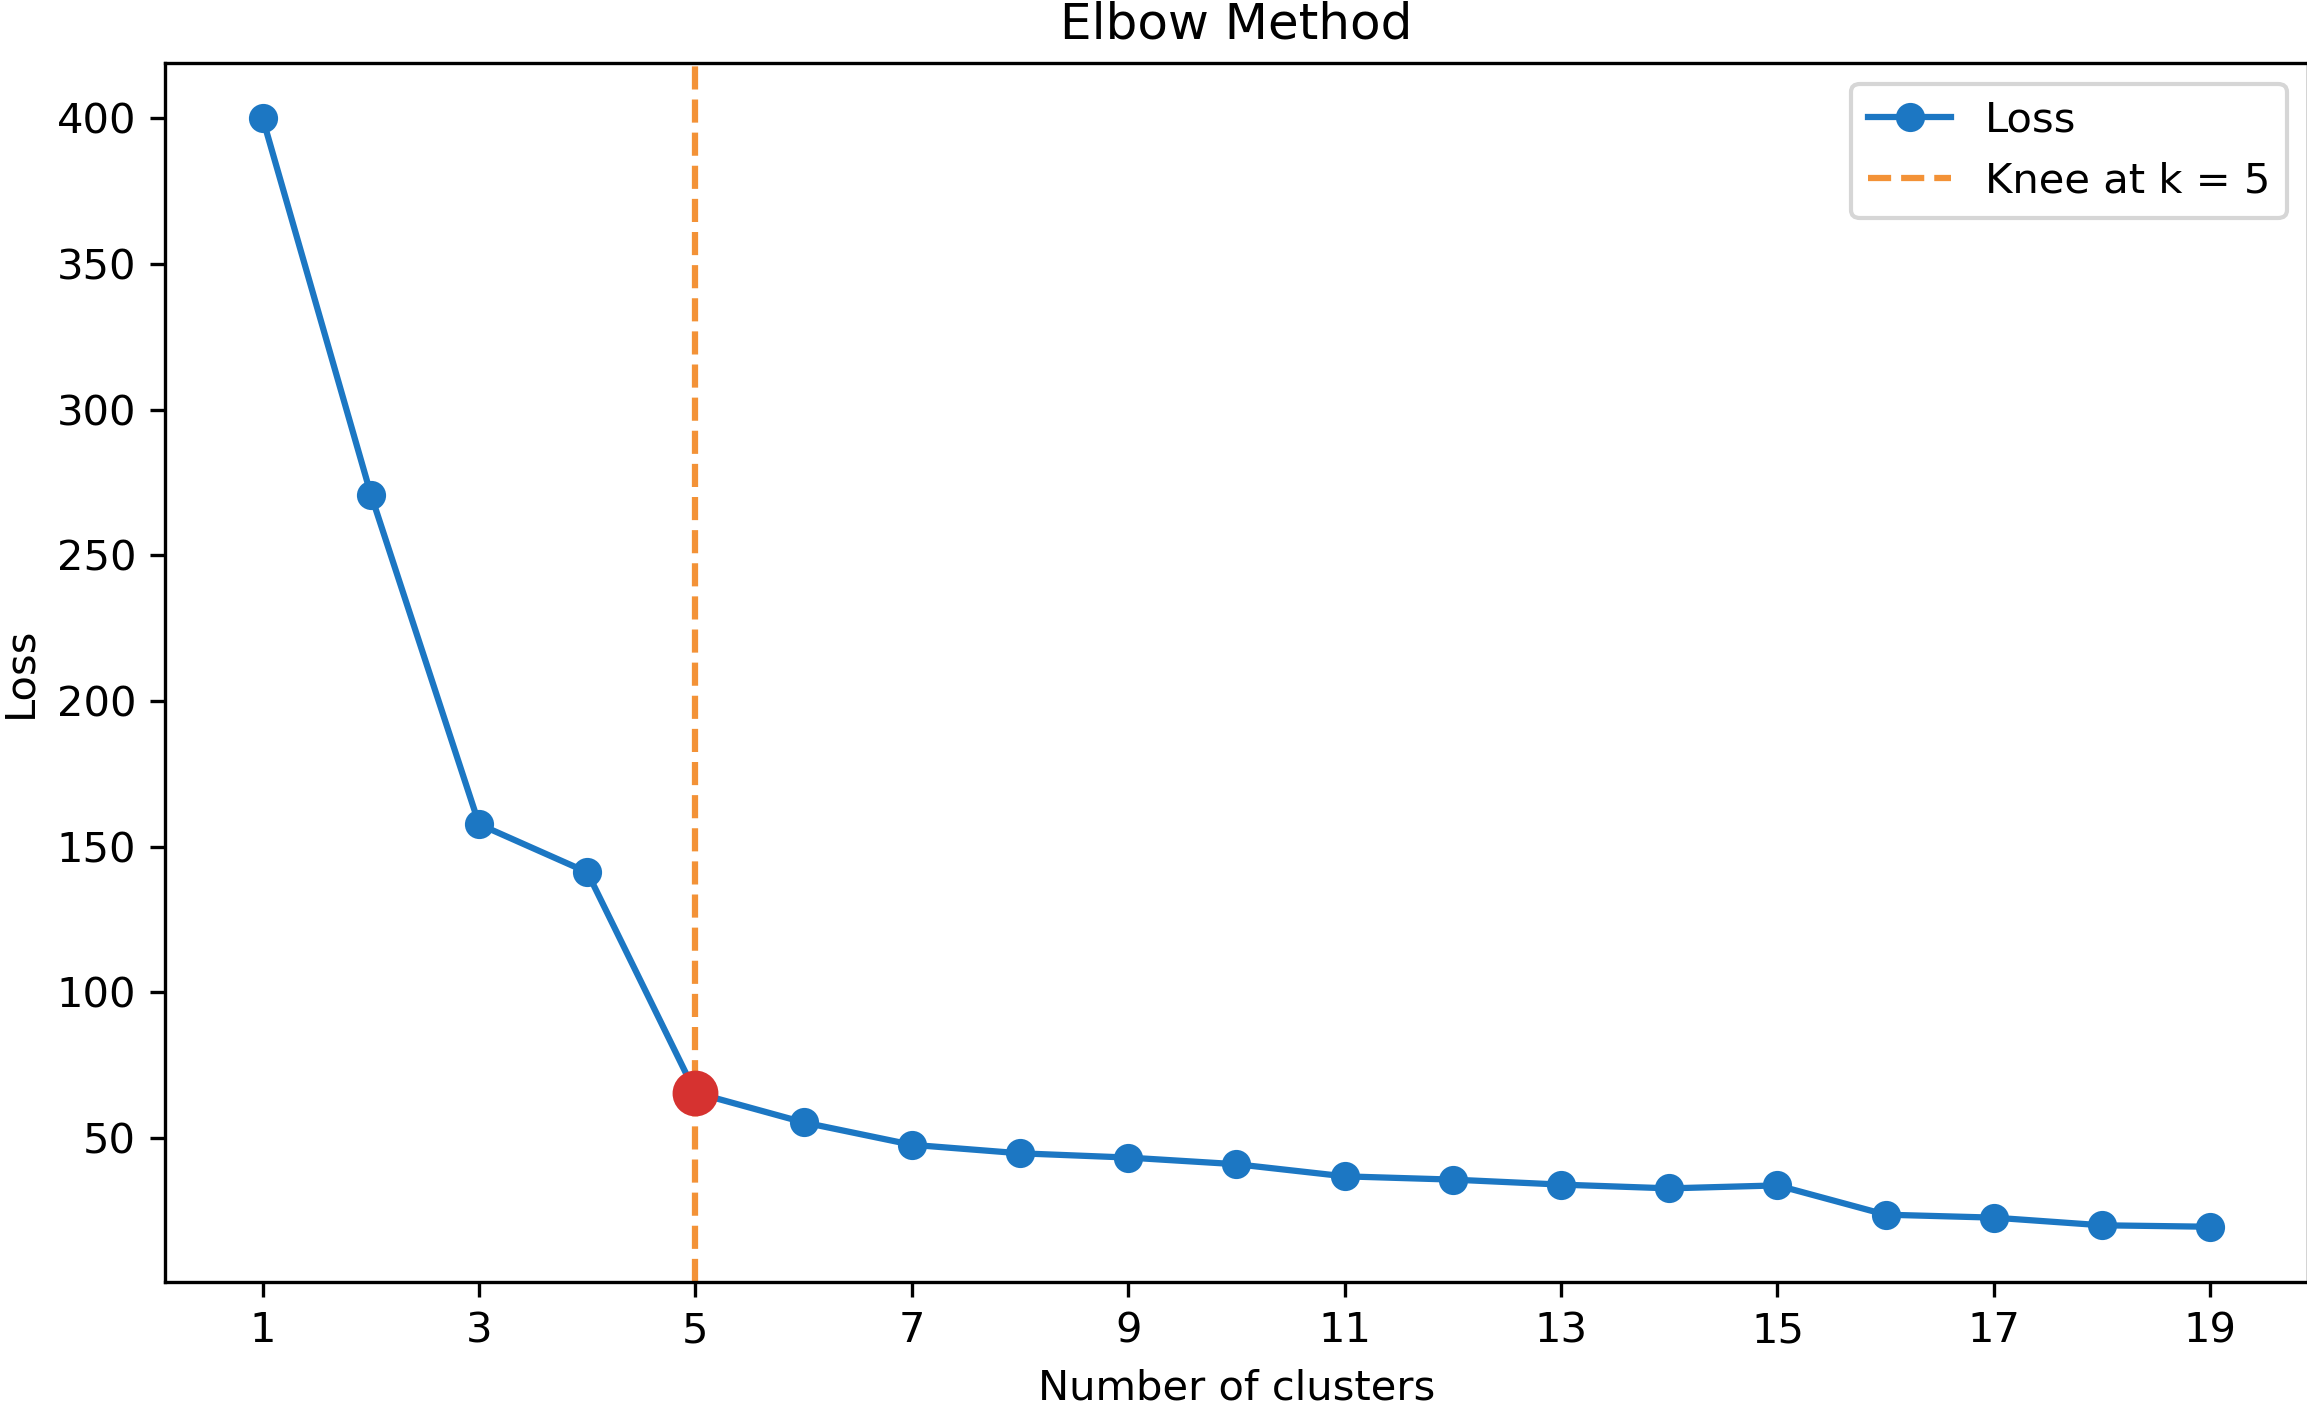
\includegraphics[width=0.9\linewidth]{figures/elbow_method}
    \end{center}
    \caption{Elbow plot using the Mall Customer Segmentation Data~\cite{KaggleMallDataset}.}
    \label{fig:elbow-plot}
\end{figure}

%------------------------------------------------------------------------

\subsubsection{Centroid initialization}

The simplest method for initializing centroids is to select them randomly.
However, as previously discussed, Lloyd’s algorithm converges to a local
minimum, making the final clustering outcome highly sensitive to the initial
centroid selection. Consequently, poor initialization can lead to suboptimal
solutions~\cite{FRANTI201995,Abdullah10601123}.

%TODO: maybe remove the numbering (1) and (2)?

According to Fränti and Sieranoja~\cite{FRANTI201995}, there are two main ways
to mitigate K-Means’ sensitivity to centroid initialization: (1) using improved
initialization techniques and (2) running the algorithm multiple times and
selecting the best result based on a predefined criterion. Several heuristics
have been proposed to enhance initialization:
\begin{itemize}
    \item \textbf{Random points} – Centroids are chosen randomly from the dataset.
    \item \textbf{Furthest point heuristic} – The first centroid is chosen randomly, and later ones are placed as far as possible from existing centroids.
    \item \textbf{Sorting heuristic} – Data points are sorted by a criterion (e.g. projection along a principal component) and used for initialization.
    \item \textbf{Density-based} – This method selects centroids in high-density regions.
    \item \textbf{Projection-based} – A dimensionality reduction technique identifies representative points for initialization.
    \item \textbf{Splitting technique} – A small number of centroids are initialized first, then iteratively refined by splitting.
\end{itemize}
Despite these efforts, \textit{"a clear state-of-the-art is
    missing"}~\cite{FRANTI201995}, meaning no single method consistently
outperforms others across all datasets. However, one widely adopted
initialization method is K-Means++, which balances randomness with a
distance-based heuristic to improve clustering performance.

%------------------------------------------------------------------------

\subsection{K-Means++}\label{subsec:k-means++}

As previously discussed, K-Means is highly sensitive to the initial choice of
centroids. K-Means++ is a widely used initialization method designed to
mitigate this issue by selecting centroids in a more systematic manner. The
algorithm follows these steps:
\begin{enumerate}
    \item Randomly select the first centroid from the dataset.
    \item Compute the distance between each data point and its nearest centroid.
    \item Select the next centroid with a probability proportional to the squared
          distance computed in step 2.
    \item Repeat steps 2 and 3 until $k$ centroids have been chosen.
\end{enumerate}
K-Means++ generally improves clustering performance by providing better initial
centroids~\cite{FRANTI201995}. However, since it still involves randomness,
suboptimal results remain possible~\cite{deuschle2019, Abdullah10601123}.

%------------------------------------------------------------------------

\section{Statistically improving K-Means}\label{sec:statistically-improving-k-means}

As noted by Fränti and Sieranoja~\cite{FRANTI201995}, K-Means presents several
opportunities for optimization. However, a key limitation is that centroids
struggle to relocate effectively when they are initially placed far from their
optimal positions. To address this issue, İhsanoğlu and
Zaval~\cite{Abdullah10601123} propose an initial solution based on simple
statistical methods, facilitating more efficient centroid movement.

%------------------------------------------------------------------------

\subsection{Identifying issues}\label{subsec:identifying-issues}

As previously mentioned, one of the main challenges in K-Means is that poorly
initialized centroids may struggle to reach their optimal positions, if at all.
This often leads to an uneven distribution of centroids — some regions may
contain too many, while others are underrepresented~\cite{FRANTI201995}. To
characterize such imbalances, İhsanoğlu and Zaval~\cite{Abdullah10601123}
propose separate approaches for \textbf{conflicting clusters} and \textbf{mega
    clusters}.

\subsubsection{Conflicting Clusters}

This type of cluster arises when multiple centroids are located too close to
one another, typically indicating redundant clustering in a dense region. To
detect them, we first compute the average distance between each centroid and
its nearest neighbour:
\begin{equation}
    \label{eq:avgDist}
    \text{AvgDist} = \frac{1}{k} \sum_{i=1}^{k} d(\mu_i, \mu_{\text{neigh}})
\end{equation}
Here, $k$ is the number of clusters, $d(x,y)$ is the distance function (e.g.
Euclidean), and $\mu_{\text{neigh}}$ denotes the closest centroid to $\mu_i$.
Using this average, we define a threshold by introducing a tunable
hyperparameter $t$. Any pair of centroids closer than $\text{AvgDist} / t$ is
considered a conflicting cluster:
\begin{equation}
    \label{eq:conflicting-cluster}
    C_i \text{ is conflicting} \iff d(\mu_i, \mu_{\text{neigh}}) < \frac{\text{AvgDist}}{t}
\end{equation}

\subsubsection{Mega Clusters}

Mega clusters, on the other hand, represent large clusters that potentially
include multiple natural groupings due to too few centroids in that region. To
detect them, we first calculate the intra-cluster variance:
\begin{equation}
    \label{eq:cluster-var}
    \text{Var}(C_i) = \frac{1}{\sum_{n=1}^{N} (r_{ni}) - 1} \sum_{n=1}^{N} r_{ni} \|x_n - \mu_i\|^2
\end{equation}
Here, $r_{ni}$ is a binary indicator showing whether point $x_n$ belongs to
cluster i, and $\|x_n - \mu_i|^2$ measures the squared distance from the data
point to the cluster centroid. The mega cluster is then defined as the cluster
with the highest variance:
\begin{equation}
    \label{eq:mega-cluster}
    C_{\max} = \underset{C_i}{\arg\max}\text{ Var}(C_i)
\end{equation}

%------------------------------------------------------------------------

\subsection{The improved algorithm}\label{subsec:the-improved-algorithm}

Based on the previously defined concepts of conflicting and mega clusters,
İhsanoğlu and Zaval~\cite{Abdullah10601123} propose an extension to K-Means
that iteratively relocates redundant centroids. The procedure is as follows:
run K-Means (or K-Means++) as usual, identify conflicting and mega clusters,
then iteratively move a centroid from a conflicting cluster to a randomly
chosen point in the mega cluster. This process is repeated until no conflicting
clusters remain or a maximum number of iterations is reached. The pseudocode
below summarizes the method:

\begin{algorithmic}[1]
    \label{alg:imprv-kmeans}
    \Require $X$, $k$, init\_func, max\_iter $ \in \mathbb{N}$, $t \in [1, \infty)$
    \State $C \gets$ \texttt{init\_func}$(X, k)$
    \State
    \For{$i = 1$ to $max\_iter$}
    \State $C,R \gets$ \texttt{converge\_to\_clusters}$(C, X, k)$
    \State
    \State $conflicts \gets$ \texttt{get\_conflicts}$(C, t)$
    \State
    \If{\texttt{len}$(conflicts) = 0$}
    \State \textbf{break}
    \EndIf
    \State
    \State $mega\_cl \gets$ \texttt{get\_mega\_cluster}$(X, k, R)$
    \State
    \State $conflict \gets$ \texttt{rand.choice}$(conflicts)$
    \State $C[conflict] \gets$ \texttt{rand.choice}$(mega\_cl)$
    \EndFor
    \State \Return $C,~R$
\end{algorithmic}

This method introduces a lightweight post-optimization step aimed at overcoming
poor initialization effects and improving cluster compactness and separation.
While simple in implementation, İhsanoğlu and Zaval report noticeable
improvements in clustering quality across various datasets.

%------------------------------------------------------------------------

\subsection{Challenges}\label{subsec:challenges}

While the improved method introduces additional statistical computations and
iterations, it differs from traditional approaches in that it does not restart
the entire clustering process. Instead, it incrementally refines an initial
K-Means result~\cite{Abdullah10601123}. This targeted adjustment increases the
likelihood of escaping poor local minima and reaching a more optimal clustering
configuration—something that is often challenging to achieve through additional
K-Means iterations alone~\cite{FRANTI201995}.

A key limitation of the approach is its dependence on the choice of the
threshold parameter~$t$. To ensure meaningful identification of conflicting
clusters, $t$ must satisfy $t > 1$; otherwise, nearly all clusters would be
classified as conflicting. Conversely, if $t$ is set too high, the algorithm
may terminate prematurely without any adjustments.

One potential strategy is to begin with a small value of $t$ and incrementally
increase it until convergence is achieved before reaching the maximum number of
iterations. However, this introduces ambiguity: early convergence could either
indicate a well-chosen threshold or that K-Means had already produced a
near-optimal solution, making it difficult to assess the effectiveness of $t$
in isolation.

%------------------------------------------------------------------------

\section{Results and Performance Evaluation}\label{sec:results-and-performance-evaluation}

Lorem ipsum dolor sit amet, consectetur adipiscing elit, sed do eiusmod tempor
incididunt ut labore et dolore magna aliqua. Ut enim ad minim veniam, quis
nostrud exercitation ullamco laboris nisi ut aliquip ex ea commodo consequat.
Duis aute irure dolor in reprehenderit in voluptate velit esse cillum dolore eu
fugiat nulla pariatur. Excepteur sint occaecat cupidatat non proident, sunt in
culpa qui officia deserunt mollit anim id est laborum.

%------------------------------------------------------------------------

\subsection{Metrics}

Lorem ipsum odor amet, consectetuer adipiscing elit. Tempor a proin quam cursus
tincidunt id fringilla. Netus hac suscipit maximus hendrerit luctus massa.
Hendrerit mollis nibh curabitur magnis netus ad diam. Sapien per conubia id
primis auctor. Porta metus feugiat tincidunt amet suscipit habitasse.

%------------------------------------------------------------------------

\subsection{Case Study: Mall Customer Segmentation}

Lorem ipsum odor amet, consectetuer adipiscing elit. Tempor a proin quam cursus
tincidunt id fringilla. Netus hac suscipit maximus hendrerit luctus massa.
Hendrerit mollis nibh curabitur magnis netus ad diam. Sapien per conubia id
primis auctor. Porta metus feugiat tincidunt amet suscipit habitasse.

%------------------------------------------------------------------------

\subsection{Measurements on different datasets}

Lorem ipsum odor amet, consectetuer adipiscing elit. Tempor a proin quam cursus
tincidunt id fringilla. Netus hac suscipit maximus hendrerit luctus massa.
Hendrerit mollis nibh curabitur magnis netus ad diam. Sapien per conubia id
primis auctor. Porta metus feugiat tincidunt amet suscipit habitasse.

%------------------------------------------------------------------------

\section{Conclusion and Future Work}\label{sec:conclusion-and-future-work}

Lorem ipsum dolor sit amet, consectetur adipiscing elit, sed do eiusmod tempor
incididunt ut labore et dolore magna aliqua. Ut enim ad minim veniam, quis
nostrud exercitation ullamco laboris nisi ut aliquip ex ea commodo consequat.
Duis aute irure dolor in reprehenderit in voluptate velit esse cillum dolore eu
fugiat nulla pariatur. Excepteur sint occaecat cupidatat non proident, sunt in
culpa qui officia deserunt mollit anim id est laborum.

%------------------------------------------------------------------------

\subsection{Summary}

Lorem ipsum odor amet, consectetuer adipiscing elit. Tempor a proin quam cursus
tincidunt id fringilla. Netus hac suscipit maximus hendrerit luctus massa.
Hendrerit mollis nibh curabitur magnis netus ad diam. Sapien per conubia id
primis auctor. Porta metus feugiat tincidunt amet suscipit habitasse.

    %------------------------------------------------------------------------

    {\small
        \bibliographystyle{ieee}
        \bibliography{kembuegler_bib}
    }

\end{document}
